Conceptually, query evaluation in PIP is broken up into two components: Query and Sampling.  PIP relies on Postgres to evaluate queries; As described in Section \ref{sec:background}, a query rewriting pass suffices to translate c-tables relational algebra extensions into traditional relational algebra.  Details on how query rewriting is implemented are provided in Section \ref{sec:implementation}.  

As the query is being evaluated, special sampling operators in the query are used to transform random variable expressions into histograms, expectations, and other moments.  Both the computation of moments and probabilities in the general case reduces to numerical integration, and a dominant technique for doing this is Monte Carlo simulation. The approximate computation of expectation
\begin{equation}
E[\chi_\phi \cdot (h \circ t)] =
\frac{1}{n} \cdot \sum_{i=1}^n p(\vec{x}_i) \cdot \chi_\phi(\vec{x}_i) \cdot
h(t(\vec{x}_i))
\end{equation}
faces a number of difficulties.  In particular, samples for which $\chi_{\phi}$ is zero do not contribute to an expectation.  If $\phi$ is a very selective condition, most samples do not contribute to the summation computation of the approximate expectation.  (This is closely related to the most prominent problem in online aggregation systems \cite{OnlineAggregation,DBO}, and also in MCDB).

The primary challenge faced by PIP is exactly this. Particularly in highly selective queries, the general-purpose sampling routines provided for each distribution will produce samples that violate query constraints $\phi$.  (This is closely related to the most prominent problem in online aggregation systems \cite{OnlineAggregation,DBO}, and also in MCDB).

\begin{example}\em 
Consider a row containing the variable 
$$[Y \Rightarrow Normal(\mu=5,\sigma^2=10)]$$
and the condition predicate $(Y > -3)$ and $(Y < 2)$.  The expectation of the variable $Y$ in the context of this row is not $5$.  Rather the expectation is taken only over samples of $Y$ that fall in the range $(-3,2)$, or about $0.17$.  
\end{example}

\subsection{Sampling Techniques}
\paragraph{Rejection Sampling}
One straightforward approach to this problem is to perform rejection sampling; sample sets are repeatedly generated until a sufficient number of viable (satisfying) samples have been obtained.  Note that this is not strict rejection sampling, samples for with $\chi_{\phi}$ is zero count towards the number or samples $n$ by which we average.  

However, without scaling the number of samples taken based on $E[\chi_\phi]$, information can get very sparse and the approximate expectations will have a high relative error.  Unfortunately, as the probability of satisfying the constraint drops, the work required to produce a viable sample increases.   Consequently, any mechanism that can improve the chances of satisfying the constraint is beneficial.

\paragraph{Sampling using inverse CDFs}
\label{subsec:icdf}
As an alternative to sampling using the generator function, PIP can use the inverse-CDF of a distribution (if available) to translate a uniform random number in the range $[0,1]$ to a variable sampled from the distribution.  The CDF increases monotonically, so to obtain samples constrained to $[lower, upper]$, we compute $CDF^{-1}(X)$ where X is chosen uniformly  from the range $(CDF(lower), CDF(upper))$.   

In the event that the inverse CDF is available, but the CDF is not, this technique may still be used.  Instead of sampling from the range $(CDF(lower), CDF(upper))$, we sample $x \in (L,H)$ where $L$ is initialized to $0$, and $H$ is initialized to $1$.  If $CDF^{-1}(x) \leq lower$ we set $L = x$ and try again.  Similarly, if $CDF^{-1}(x)  \geq upper$ we set $H = x$ and try again.   In this way, PIP effectively learns the values of $CDF(lower)$ and $CDF(upper)$.  

If precise bounds can be derived from the constraints on a given variable, this process guarantees that each sample generated will satisfy the constraint.  Even if only weak bounds are available, the process still provides a benefit.  By reducing the size of the sampling area, the probability of selecting a viable sample is still increased.  

\paragraph{Exploiting independence}
\label{subsec:independence}
Viable samples are also encountered with higher frequency when the number of variables being constrained is smaller.  Fewer variables mean less work is lost when a sample is rejected.  Similarly, fewer constraints mean a lower overall chance of rejection.  PIP exploits this by first subdividing constraint predicates into minimal independent subsets.  Two constraint subsets are independent if their member predicates have no variables in common.  When determining subset independence, composite random variables (for instance, defined by artithmetic expressions over random variables) are treated as the set of all of their component variables.  Note that two variables may appear in the expectation function and still be considered independent; only the selection predicates are considered when determining independence.

By definition, variables in each set are independent.  Thus, the probability of each subset may be computed independently as well; the overall probability is the product of the independent probabilities.  For example, consider the one row c-table 
\[
\begin{tabular}{c|c}
R & $\phi_2$ \\
\hline
& $(X > 4) \wedge ([X\cdot Z] > Y) \wedge (A < 6)$ \\
\end{tabular}
\]
In this case, the atoms $(X > 4)$ and $([X\cdot Z] > Y)$ form one minimal independent subset, while $(A < 6)$ forms another.

Condition atoms describing discrete variables are all of the form $Var = Val$, discrete variables are handled trivially.  Inconsistent values have already been removed, so the probability for the entire subgroup is the probability of the listed variable assignment.

The simplest subset of continuous atoms is one that references only one variable.  In this case, the atoms in the set provide constant upper or lower bounds, and the integration problem may be solved by evaluating the variable's CDF at the tightest upper and lower bounds.  If the CDF is not available or if it is not possible to derive tight bounds on the CDF, PIP can still integrate via Monte Carlo sampling.  

\paragraph{Metropolis}
A final alternative available to PIP, is the
Metropolis  algorithm \cite{metropolis}.   Starting from  an arbitrary
point within the sample space,  this algorithm performs a random walk.
Steps  are  sampled  from  a  multivariate  normal  distribution,  and
rejection sampling  is used  to weight the  walk towards  regions with
higher  probability  densities.  Samples  taken  at regular  intervals
during the random walk may be used as samples of the distribution.

The Metropolis algorithm has an  expensive startup cost, as there is a
lengthy  `burn-in' period  while  it generates  a sufficiently  random
initial  value.  Despite  this startup  cost, the  algorithm typically
requires only a relatively small  number of steps between each sample.
Consequently,   the  Metropolis  algorithm   is  ideally   suited  for
generating large numbers of samples  when the CDF is not available and
the probability of sampling a given value is small.

%{\bf Integration}
%
%There are  cases where bounds are insufficient.   For example, concave
%atoms  are   not  likely   to  admit  effective   rectangular  bounds.
%Similarly, even though a bounding box  covers no less than half of the
%volume of a contiguous convex constraint area, the  bulk of the  probability mass may
%still lie  outside of the constrained  sample area.  In  such cases, a
%recursive technique may be applied.
%
%The  bounding box  is first  subdivided into  smaller  regions.  Monte
%Carlo integration  is performed on the  region twice, but  with only a
%small number of iterations apiece.  If the two results agree to within
%the  desired  precision, integration  stops  and  the  average of  the
%results is multiplied by the  probability of a sample falling into the
%sampling region.  If the  two results differ significantly, the region
%is further subdivided and the algorithm recurses on each sub-region.
%
%Because the  recursive cutoff is determined by  the estimated accuracy
%of the  result, this  algorithm will not  recurse on regions  that are
%entirely   within  or   outside  of   the  constrained   sample  area.
%Consequently, the majority of  samples generated by the algorithm will
%be  put towards estimating  relatively high  values where  Monte Carlo
%integration is most effective.


\subsection{Sampling Operators}
After a query has been evaluated on probabilistic data, what remains is another set of probabilistic data.  To permit analysis of this data, PIP provides a set of sampling operators: functions that convert probabilistic data into deterministic metrics.  These operators take in an expression to be evaluated and the expression's context, or boolean formula of constraints associated with the expression's row and output a histogram, expectation, or higher moment for the expression under the constraints of its context.  As described in Section \ref{sec:background}, without loss of generality, it is possible to express the context as a set of conditions to be combined conjunctively.  

These basic sampling operators follow \textit{per-row sampling semantics}.  The metric in question is taken over only the volume of probability space defined by the expression's context.  For example, in the case of Monte-Carlo sampling, only samples satisfying all of the context's conditions are considered.  All other samples are discarded, not even counting towards the net value.  If the context is contradictory, a value of NAN will result.

Note that the resulting metrics are still probabilistic data; The metric being computed is valid for the variable expression in the context of the row, but the row is still only present in the database for variable valuations satisfying the row's context.  The conf operator is used to obtain the probability of a satisfying valuation, a value known as the row's confidence.  If the conf operator is present, all conditions applying to the row are removed from the result and the resulting table is deterministic.


%%%%%%%%%%%%%%%%%%%%%%%%%
The sampler computes the expression's expectation by first subdividing the problem to exploit independence.  These groups are subsequently divided into two categories: Groups containing at least one variable contained in the target expression are marked for sampling.  The volume of the probability space defined by all constraints must be computed, but storage overheads may be avoided for those groups not directly relevant to the target expression; these groups are marked for integration.  Additionally, if such a group contains only one variable, the integral may be computed exactly using a single call to the variable's CDF if one is available.

The remaining groups are sampled to obtain values for Monte-Carlo estimation of the target expression's expectation.  By default, these samples are obtained through naive rejection sampling.  Variables are selected from the distribution $\frac{\chi(\vec{x})p(\vec{x})}{\int_{\vec{a}} \chi(\vec{a})p(\vec{a})}$ by sampling according to $p(\vec{x})$ and discarding values that do not satisfy $\phi(\vec{x})$.  Finally, the expectation value computed is re-normalized according to the frequency with which samples are discarded.

If any of the variables have a CDF available, PIP first attempts to obtain weak bounds on the variable as described in Section \ref{subsec:icdf}.  If such bounds are available, PIP can use the variable's CDF and inverse CDF to restrict sampling to within the weak bounds.  If the weak bounds are actually tight bounds, no samples will be discarded.  However, even if some samples are rejected, the bounds reduce the drop frequency.  When computing the volume of the probability space defined by the constraints, the values are re-normalized according to the fraction of the CDF located within the bounds.

A final option available to PIP is the Metropolis algorithm.  Metropolis has a high initialization cost: Prior to sampling, at least one value $\vec x$ satisfying $\theta(\vec x)$ must be found (though it need not be selected according to any specific probability distribution), and a significant number of burn-in iterations must be run and discarded.  Furthermore, every sampling step requires many Metropolis iterations to achieve sufficiently independent samples.  However, Metropolis is guaranteed to stay within the constraint bounds and no samples will be rejected.  Thus, we can estimate the work required for both Metropolis and Naive rejection sampling.

$$W_{metropolis} = C_{burn\ in} + [\#\ samples] \cdot C_{steps\ per\ sample}$$
$$W_{naive} = \frac{1}{1-P[reject]} \cdot [\#\ samples]$$

By generating a small number of samples for the subgroup, PIP generates a rough estimate of $P[reject]$.  If this value is lower than $\frac{1}{\frac{C_{burn\ in}}{[\#\ samples]} + C_{steps\ per\ sample}}$, Metropolis sampling is used instead of rejection sampling.  Note that if CDFs are available for one or more component variables, PIP uses the probability of rejecting samples chosen from within the available weak bounds.

The single-row sampling process is sumarized in Figure \ref{fig:roadmap}

\begin{figure}
\begin{center}
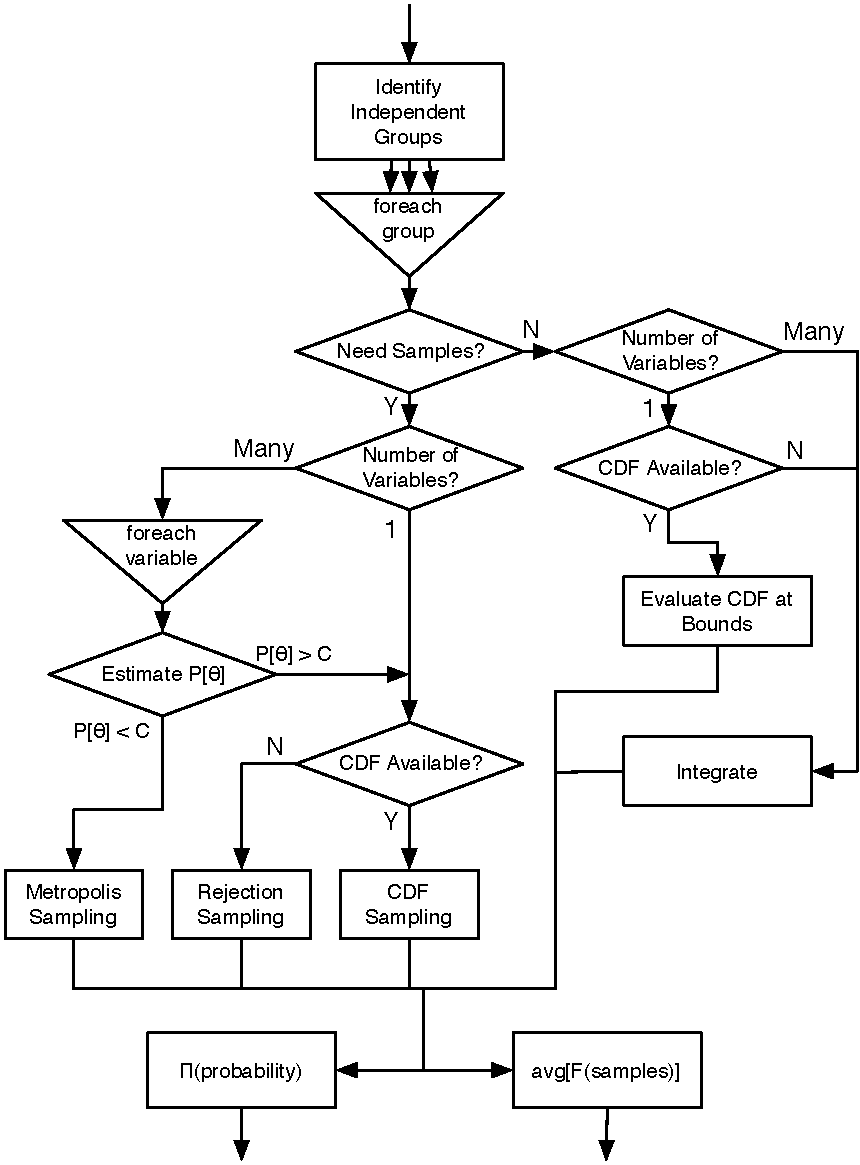
\includegraphics[width=3in]{graphics/roadmap.pdf}
%\begin{enumerate}
%\item 
%\end{enumerate}
\caption{\textbf{The PIP Single-Row sampling process}}
\vspace*{-0.2in}
\label{fig:roadmap}
\end{center}
\vspace*{-0.15in}
\end{figure}

\subsection{Aggregate Sampling}
The complexity introduced by aggregate operations, coupled with the frequency with which they appear at the root of a query plan, makes them an ideal point at which to perform sampling.  We begin with the simplest form of aggregate expectation, that of an aggregate that obeys linearity of expectation ($\left<f(\vec{x})\right> = f(\vec{\left<x\right>})$), such as sum().  

Such aggregates are straightforward to implement: per-row expectations of $f(\vec x)\chi(\vec x)$ are computed, and aggregated (e.g., summed up).  Of note however, is the effect that the operator has on the variance of the result.  In the case of sum(), each expectation can be viewed as a Normally distributed random variable with a shared, predetermined variance.  By the law of large numbers, the sum of a set of $N$ random variables with equal variance $\sigma$ has a variance of $\frac{\sigma}{\sqrt{N}}$.  In other words, when computing the expected sum of $N$ variables, we can reduce the number of samples taken for each individual element by a factor of $\frac{1}{\sqrt{N}}$.

If the operator does not obey linearity of expectation (e.g., computing the maximum), either the aggregate must be designed with expectation computation in mind, or the aggregate must be run on a set of sampled worlds in parallel.  This latter technique is a worst-case approach to the problem; it may be necessary to re-run the aggregate if an insufficient number of sample worlds are generated. Note however, that this is still more efficient than re-running the entire query.

The max() aggregate can be implemented more efficiently, particularly when the target expression is a constant (ie, a value that is certain for the row in question).  Given a table table sorted over descending values of the target expression, PIP estimates the probability that the first element in the table (the highest value) is present.  The aggregate expectation is initialized as the product of this probability and the first element.  The second term is maximal only if the first term is not present; when computing the probability of the second term, we must compute the probability of all the second term's constraint atoms being fulfilled while at least one of the first atom's terms is not fulfilled.  Though the complexity of this process is exponential in the number of rows, the probability of each successive row being maximal drops exponentially.  




